\section{Evaluation}
\label{sec:evaluation}

\begin{figure*}[htbp]
\centering
\begin{minipage}{.63\textwidth}
\begin{subfigure}{0.5\textwidth}
    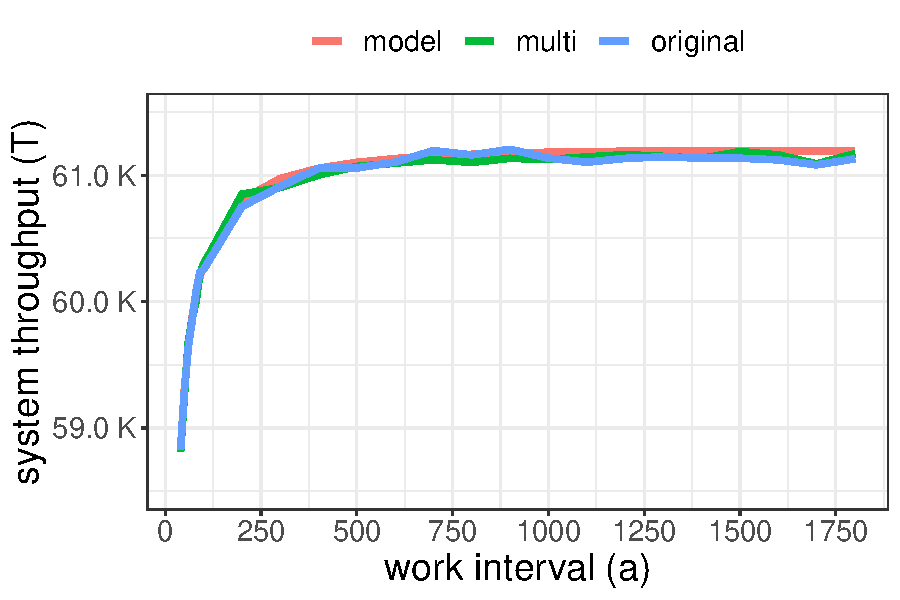
\includegraphics[width=\linewidth]{figures/fig-4a.pdf}
    \caption{System throughput $vs.$ $a$ in $ms$.} \label{fig:4a}
  \end{subfigure}%
  \hspace*{\fill}   % maximize separation between the subfigures
\begin{subfigure}{0.5\textwidth}
    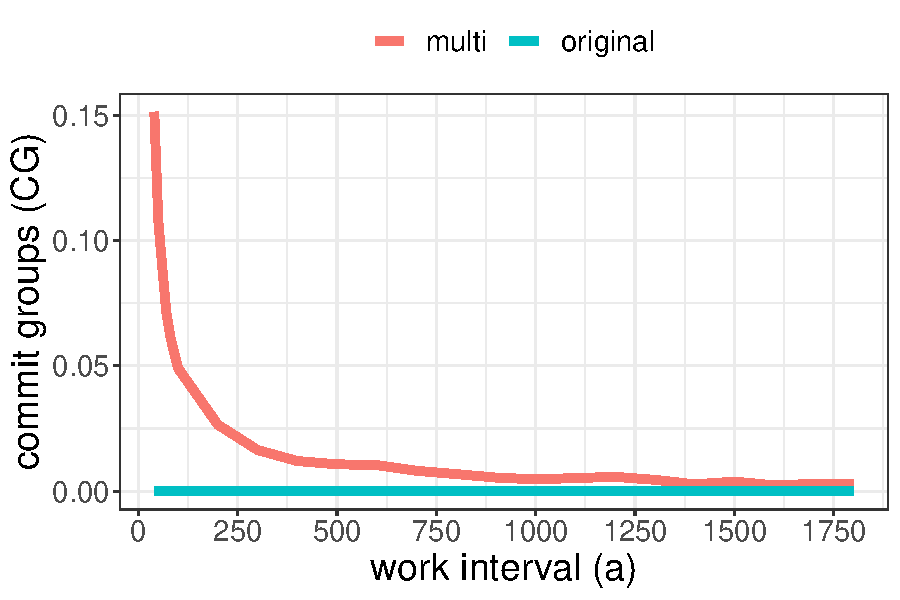
\includegraphics[width=\linewidth]{figures/fig-4b.pdf}
    \caption{Operational commit groups $vs.$ $a$ in $ms$.} \label{fig:4b}
  \end{subfigure}
\caption{Maximum throughput as work interval $a$ varied from 40 to 1800 $ms$.} \label{fig:4}
\end{minipage}\hfill
\begin{minipage}{.35\textwidth}
  \centering
  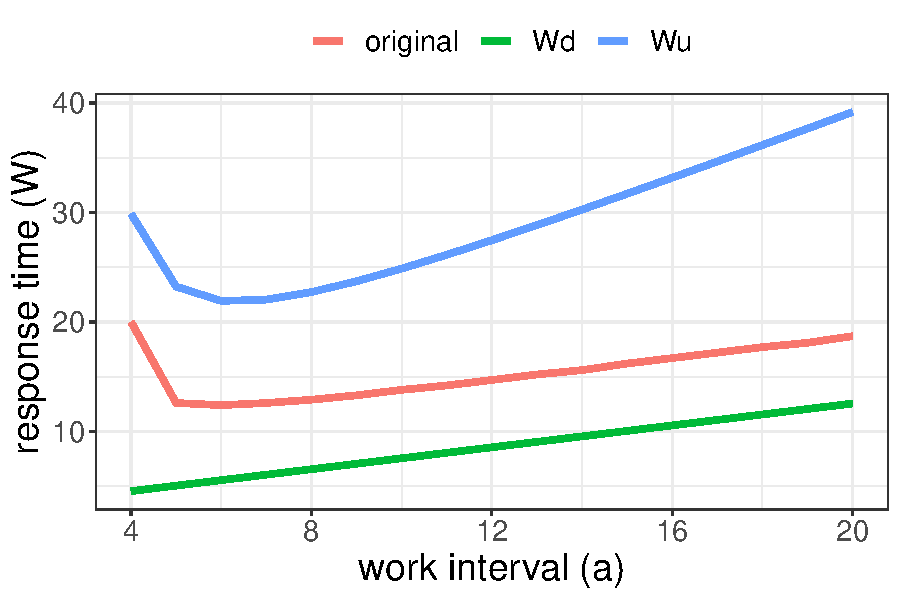
\includegraphics[width=0.8\linewidth]{figures/fig-5.pdf}
  \caption{Average response time ($ms$) in epoch-based commit \textit{vs}. $a$ in $ms$.
  }
  \label{fig:5}
\end{minipage}
\end{figure*}



% In this section, we study the performance of both the epoch-based
% commit\footnote{Referred to as \emph{original} in figures.} and multi-commit
% protocols.
% Specifically, we focus on the following questions:
% \begin{itemize}
% \item What are the optimal work intervals that maximize throughput and minimize transactions' average response time?
% \item How accurate are the approximate models in~\Cref{sec:epoch-based-commit} for
%   estimating the optimal work interval when compared to simulations?
% \item What are the performance benefits of epoch-based multi-commit?
% \end{itemize}

Each simulation run took approximately 12 hours to complete and simulated a cluster operational period of 100 
days in order to have thousands of cycles with node failures. (Note: Experiments in~\cite{lu} did not study the impact of node failures.) For example, when $a=40~ms$, 10,972 cycles had 
failures out of a total of 207 million cycles simulated. So, the number of operational commit groups reported 
here would be an average of at least 10,000 values obtained. 
We observed up to 10 cycles having multiple node failures when $a=1800~ms$.
%; that is, some node failed every 5.33 (simulated) hours during the 100 day period. This matches the theoretical expectation: when the failure intervals for each node is exponentially distributed with mean = $1/ \xi = 12$ hours, the first of the 64 nodes fails in  $64 \xi$, given the memoryless nature of the distribution. 

\subsection{Maximum Throughput}
\label{sec:determ-optim-ep}

\Cref{fig:4a} plots the maximum attainable throughput values against the work interval $a$ which is varied 
from 40 to 1800 $ms$. Throughput estimated using the expression in~\Cref{sec:maximum-throughput} is referred 
to as \emph{`model'} and those measured in simulations for epoch-based commit and epoch-based multi-commit 
are labelled as \emph{`original'} and \emph{`multi'} respectively. Simulations used the random assignment 
policy when a distributed transaction sought to interact with a remote node.

We can make three observations from~\Cref{fig:4a}. First, the estimated throughput very closely tracks the 
simulated values at all $a$. In fact, the maximum difference ever observed was around 3.8\%.
%($\thicksim2,300~T$).
This suggests that Assumptions 1 and 2 of~\Cref{sec:model-assumptions} have a 
negligible impact on the accuracy and the analytical model is nearly exact. 

Secondly, throughput values of both protocols are nearly identical. This is explained by 
\Cref{fig:4b} that presents the number of operative commit groups ($CG$) formed in cycles with node failures. 
$CG$ takes the maximum value of just $0.15$ and rapidly falls as $a$ increases. Such insignificantly 
small values of $CG$ in multi-commit are due to the proportion of distributed transactions (10\%) in the 
workload and the random policy employed for choosing the node to interact with. These two factors lead to 
almost all operative nodes interacting, directly or indirectly, with the failed node by the time the work 
interval $a$ completes. This effect is more pronounced for larger $a$ values. Consequently, multi-commit 
cannot perform significantly better than the original when nodes fail. Moreover, even this minute performance 
advantage of multi-commit during cycles with failures nearly vanishes when average throughput is 
taken over all cycles, because failure-free cycles far out-number those with failures. (Recall, when 
there are no failures, multi-commit performance is identical to the original.)

Finally, the analytical expression of \Cref{sec:maximum-throughput} can be reliably used in choosing 
appropriate $a_T$ when maximum throughput is the primary concern. For convenience, \Cref{fig:4a} is 
reproduced in Appendix as \Cref{fig:7} without simulated throughput values so that throughput 
estimates for various $a$ are clear. Referring to \Cref{fig:7}, we observe that  throughput does not 
decrease until $a=1500~ms$; thus, optimal $a_{T}^*$ is $1500~ms$. For some workloads, a work interval around 
$1500~ms$ will offer unsatisfactory latency and be unacceptable. Thus, finding a smaller $a_T$ that still 
offers an acceptable maximum throughput may be desirable and can be guided by the observation that increasing 
$a$ need not fetch a proportional increase in throughput. \Cref{fig:7} shows four distinct regions 
where the rate of throughput increase is markedly different: the gradient is very large, fairly large, small 
and very small when $a \in [40, 100)$, $a \in [100, 300)$, $a \in [300, 500)$ and $a \in [500, 1500] ~ms$  
respectively. 

\subsection{Average Response Time}

Our second set of experiments focus on assessing the effectiveness of the average response time analytical 
models in \Cref{subsec:upperbound,subsec:lowerbound}. Simulations retain the random assignment policy for 
distributed transactions; transaction arrival rate per second is taken to be $\lambda = 30,000$ which is 
approximately 90\% 
of the maximum throughput when $a = 5ms$ to ensure the system is in a steady state. \Cref{fig:5} plots the 
model estimates of the lower ($W_d$) and upper bounds ($W_u$) and the simulation values measured for 
epoch-based commit protocol as $a$ is varied from 4 to 20 $ms$. (The range choice for $a$ is guided
by~\cite{lu} where experiments used $a = 10 ~ms$.)

The response times measured in simulations are well within the upper and lower bound estimates. The latter 
increase linearly with $a$ as expected. The $W_u$ plot predicts the optimum $a$ for minimising the average 
response time as: $a^{*}= 6 ~ms$ which is consistent with simulations.
Though the analytical expression for $W_u$ (\Cref{subsec:upperbound}, \Cref{Wu}) identifies $a^{*}$ 
reasonably accurately, the actual response times are much closer to $W_d$ as $a$ increases and the maximum 
difference we observed was 6 $ms$. % 53% difference
So, to summarise, analytical expressions for $W_u$ and $W_d$ are reasonably accurate in predicting $a^{*}$ 
and the actual response times for $a \geq a^{*} $ respectively. The simulation response times obtained for 
multi-commit were very close to those presented for the original for reasons explained in 
\Cref{sec:determ-optim-ep} and hence they are not shown. 

% It is visible that $W_u$ over-estimates the average response time, but it
% does indicate the same optimal work interval as the simulation.
% Whereas $W_d$ consistently underestimates the latency by around 6$ms$ and 
% does not indicate $a^{*}$.
% Together $W_u$ and $W_d$ can be used to garner a good estimate of the expected
% average response time. 
% Lastly, \Cref{fig:5} demonstrates that the optimal work interval differs 
% greatly depending on whether the user desires optimal latency or throughput.

\begin{figure*}
\centering
\begin{subfigure}{.32\textwidth}
    \centering
    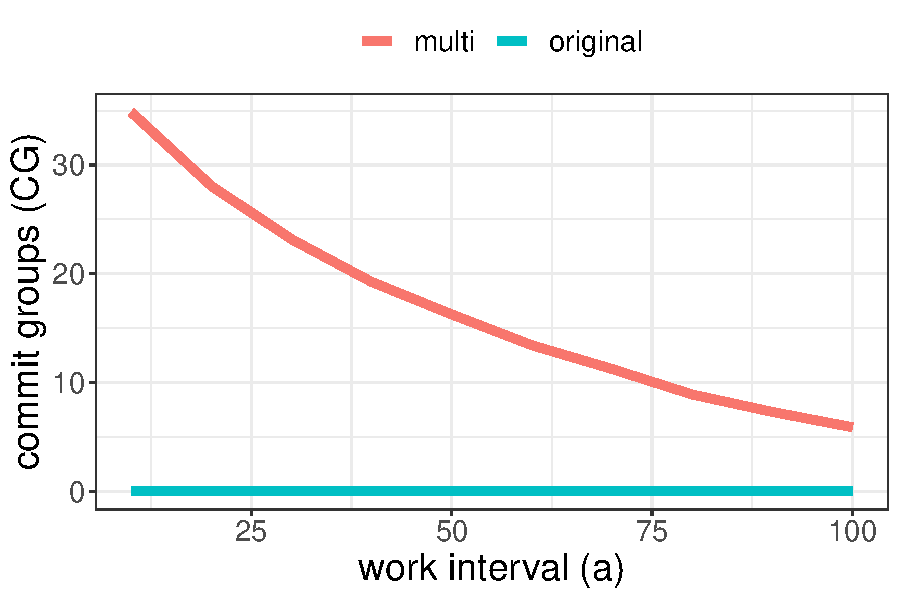
\includegraphics[width=.95\linewidth]{figures/fig-6a.pdf}  
    \caption{Commit groups $vs.$ $a$.}
    \label{fig:6a}
\end{subfigure}
\begin{subfigure}{.32\textwidth}
    \centering
    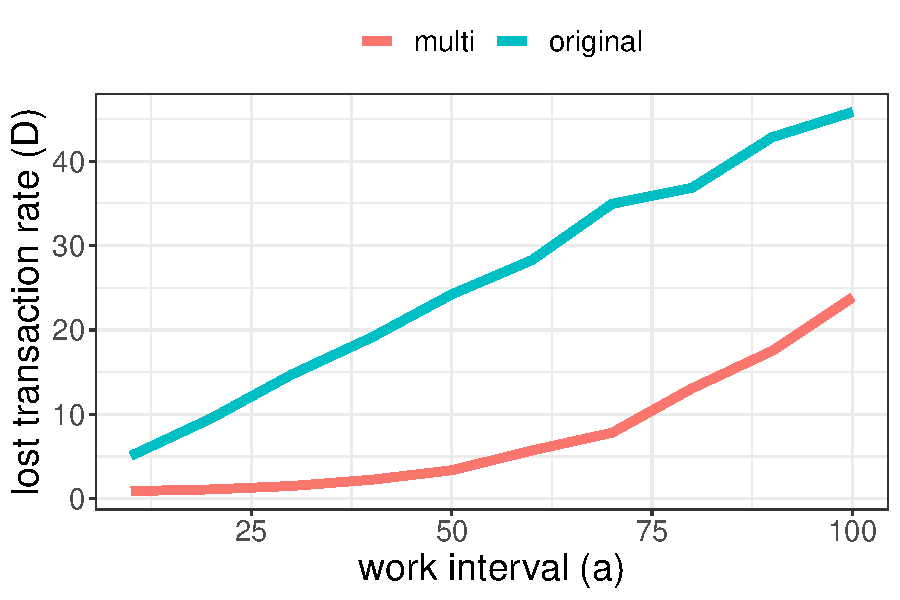
\includegraphics[width=.95\linewidth]{figures/fig-6b.pdf}  
    \caption{Lost transaction rate $vs.$ $a$ in $ms.$}
    \label{fig:6b}
\end{subfigure}
\begin{subfigure}{.32\textwidth}
    \centering
    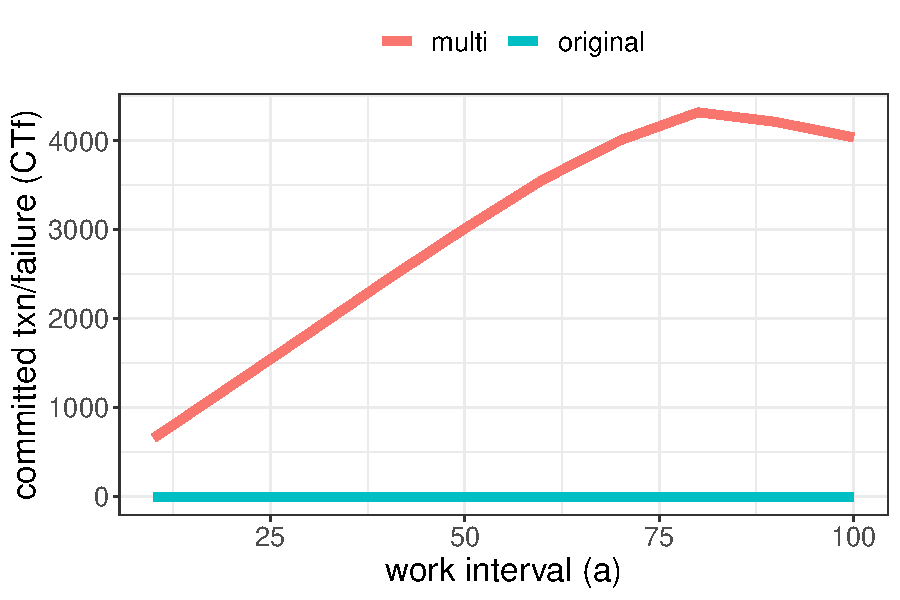
\includegraphics[width=.95\linewidth]{figures/fig-6c.pdf}  
    \caption{Average number of transactions committed in cycles with node failure $CT_f$ $vs.$ $a$.}
    \label{fig:6c}
\end{subfigure}
\caption{Simulations under paired-affinity as work interval $a$ varied from 10 to 100 $ms$.}
\label{fig:6}
\end{figure*}

\subsection{Paired Affinity}
\label{sec:trans-saved-per}

% In~\Cref{fig:4}, epoch-based multi-commit offers no obvious benefits over epoch-based commit.
% We now analyze the conditions under which multi-commit improves performance.
% Recall, multi-commit aims to avoid unnecessarily discarding completed transactions in
% the event of a node failure, thus it would be anticipated that the lost transaction rate would be lower 
% compared to normal epoch-based commit.
% The main determinant behind saving completed transactions is the number of commit groups that can be formed in
% an epoch, and the number of these which are operational at commit time; 
% in \Cref{fig:4b} it is almost 0, hence no performance gain.
% In epoch-based commit there is always a single commit group, thus if one member
% fails then all non-failed members must also discard their completed transactions.
% The number of commit groups is influenced by three workload characteristics:
% (i) the proportion of distributed transactions,
% (ii) the number of remote nodes they access
% and (iii) \emph{node affinity}, that is, groups of nodes that are more likely to be
% accessed within the same transaction owing to correlations in the underlying data.

We ran the maximum throughput simulation experiment using the paired affinity selection policy for distributed
transactions. \Cref{fig:6a} displays the number of operational commit groups ($CG$) formed whenever failures
occurred in a cycle. In sharp contrast to~\Cref{fig:4b}, $CG$ for multi-commit starts at a much larger 
value of $35$ when $a=10 ~ms$ and falls steadily to $5$ as $a$ increases to $100 ~ms$. This suggests a strong 
potential for reducing the number of aborts when failures occur. 

\Cref{fig:6b} plots the lost transaction rates ($D$) for both protocols and shows that $D$ for multi-commit 
is consistently smaller than the original. 
For small $a$, the difference is small, because the number of transactions lost due to failures is small for both
protocols.
% The difference is small for small values $a$ as the number of transactions lost due to failures is also small for the original, epoch-based commit. 
But as $a$ increases, $D$ for the original increases almost linearly while that for multi-commit does not 
start increasing significantly until $a=50~ms$; at that point, multi-commit shows 83\% reduction in $D$ with 
the corresponding $CG$ being around $17$ in~\Cref{fig:6a}. As $a$ increases further, $CG$ for multi-commit 
starts dropping significantly in~\Cref{fig:6a} and consequently $D$ for multi-commit starts increasing rapidly.
%For $a$ increases beyond $100 ~ms$, larger than approaching $D$ for the original in~\Cref{fig:7}.  

Finally, \Cref{fig:6c} shows the average number of transactions committed by the protocols in those cycles 
where node failures occur ($CT_f$). 
From \Cref{fig:6c} it is clear that multi-commit avoids a significant 
number of aborts; note that $CT_f = 0$ in the original. %, as all transactions are discarded when a node fails.
However, these differences in $CT_f$ make insignificant difference when 
throughput and latency are averaged over the simulation period,  
because cycles without failures far outnumber (by four orders of magnitude) those with failures and both protocols perform identically in fail-free cycles. 
Thus, the average maximum throughput and average
latency for both protocols, plotted in \Cref{fig:8a,fig:9a} (in Appendix), are almost identical. 
This implies
% also means 
that 
the analytical expressions obtained for epoch-based commit under the random policy have a wide applicability:
comparing Figures \ref{fig:8a} and \ref{fig:9b} with Figures \ref{fig:8b} and \ref{fig:5}
respectively suggests that those expressions are equally applicable for (i)
obtaining appropriate $a$ for epoch-based multi-commit, and (ii) epoch-based protocols under paired affinity policy. 
%for the desired performance targets of throughput and/or average latency.  
% This is reflected in the number of operational commit groups, which is around 17,
% hence within each epoch a significant number of nodes are still able to commit their
% completed work if a failure event occurs.